% Section content template for individual Educative lessons
% This file contains the actual content for a specific section
% Generated from Educative API section content

% Section: Introduction to a CDN
% Section ID: 5560114131501056
% Section Slug: introduction-to-a-cdn
% Generated: 2025-12-07T17:13:06.875311

A content delivery network (CDN) is a distributed system of servers placed in many geographic locations to improve the speed and reliability of delivering online content. Rather than relying on a single origin server that holds the original version of the data, a CDN uses a network of proxy servers positioned closer to users. When requests arrive, these nearby servers act as intermediaries, providing content on behalf of the origin server. This setup reduces the load on the origin server and helps protect it from traffic spikes and potential attacks.
\\
The proxy servers are placed at the network edge(The network edge is the zone where a device or local network interfaces with the Internet.) and are often called edge servers. By storing copies of content near end users, edge servers reduce latency, save bandwidth, and deliver data more quickly. A basic proxy simply forwards requests, but a CDN adds intelligence that optimizes how and where content is delivered.
\\
The guiding idea behind a CDN is to minimize the distance that data must travel to reach the user. To achieve this, CDNs place small data centers near users and store copies of the required content there. By storing both static(This type of data doesn't change frequently and remains on the servers for a long period.) and dynamic(This type of data changes most frequently---for example, newsletters, ads, live videos, and so on.) content close to end users, CDNs can significantly reduce propagation delay, which is the time it takes for data to travel across the network. They also work to reduce transmission and queuing delays by ensuring that sufficient bandwidth is available along the delivery path, often within the user's ISP.
\begin{quote}
\textbf{Note}: Cache is often confused with CDN. Cache is a local storage method for frequently used data, while a CDN spreads content across multiple locations to reach users faster and more reliably.
\end{quote}
\\
Let's look at the different ways CDN solves the discussed problems:

\begin{itemize}
\item
\protect\phantomsection\label{kfD2ZIt3n3dQCpN7Z9sur}
\textbf{High latency}: A CDN brings content closer to end-users via edge servers, reducing the physical distance data travels and improving response times. This also reduces network congestion and propagation delays.
\item
\protect\phantomsection\label{c8627ljQvLkX7nZApCMLQ}
\textbf{Data-intensive applications}: Since the path to the data includes only the ISP and the nearby CDN components, there's no issue in serving a large number of users through a few CDN components in a specific area. As shown below, the origin data center will need to provide the data to local CDN components only once, whereas local CDN components can then provide the data to different users individually. No user will have to download their own copy of data from the origin servers.
\end{itemize}
\begin{quote}
\textbf{Note}: Various streaming protocols are used to deliver dynamic content by the CDN providers. For example, CDNsun uses the Real-time Messaging Protocol (RTMP), HTTP Live Streaming (HLS), Real-time Streaming Protocol (RTSP), and many more to deliver dynamic content.
\end{quote}
\begin{itemize}
\item
\protect\phantomsection\label{VQOC8JG7RzAdRROvvuu6S}
\textbf{Scarcity of data center resources}: A CDN is used to serve popular content. For this reason, most traffic is handled at the CDN instead of the origin servers. So, different local or distributed CDN components share the load on origin servers.
\end{itemize}

\begin{figure}[htbp]
 \centering
 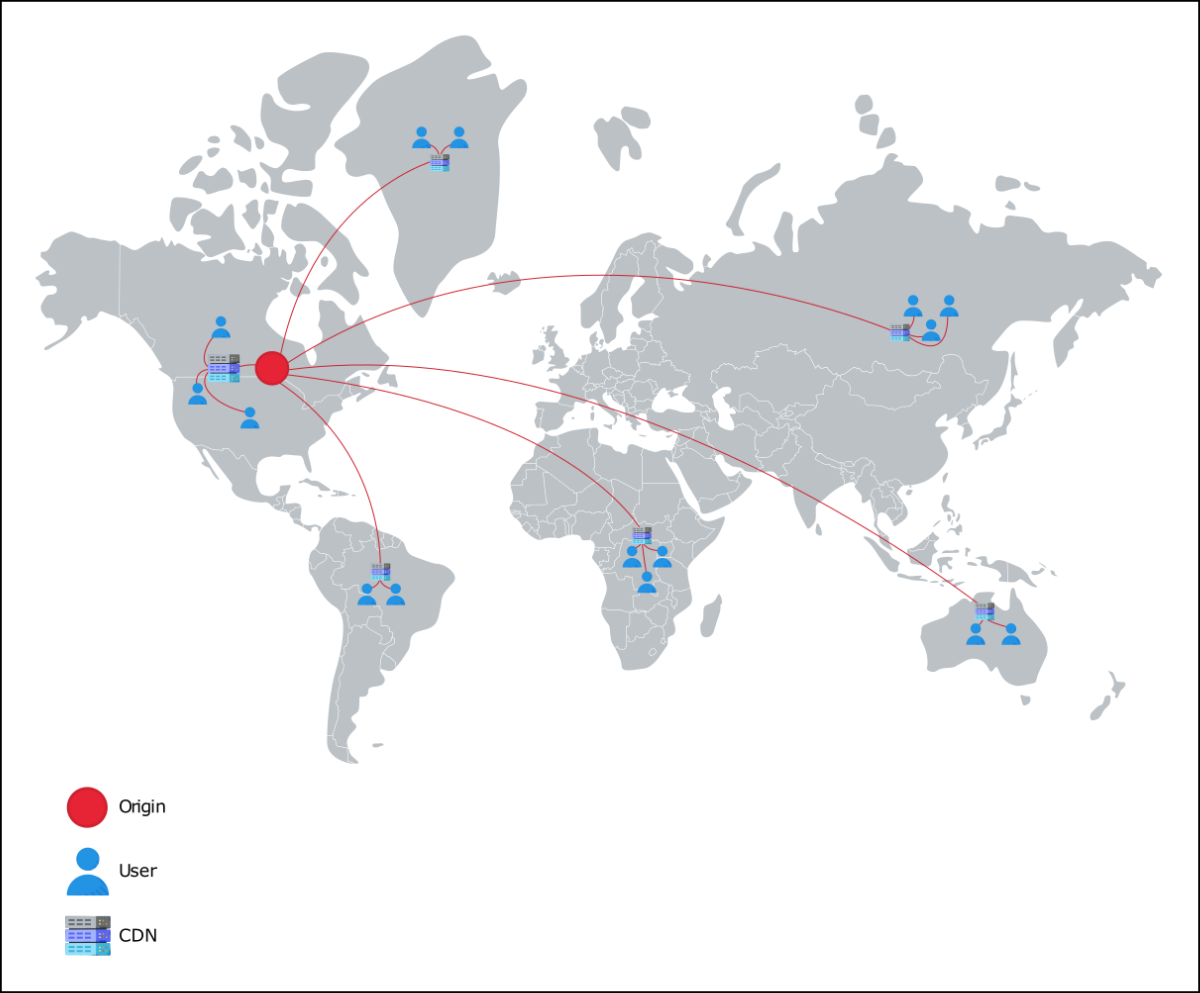
\includegraphics[width=0.5\textwidth]{Images/chapter_11/section_5560114131501056/4800748351520768.png}
 \caption{Dissemination of content to a geographically distributed CDN}
\end{figure}

\begin{quote}
\textbf{Note:} A few well-known CDN providers are Akamai, StackPath, Cloudflare, Rackspace, Amazon CloudFront, and Google Cloud CDN.
\end{quote}

\begin{quote}
\textbf{Quiz:}
\textbf{Question 1:} Does a CDN cache all content from the origin server?
\textbf{Answer:} Not likely. A CDN caches a considerable portion of the content depending on its capabilities, and it mostly caches the static content:

The content that isn\textquotesingle t frequently changed is known as static content. It also depends on the size of the content. For example, it might be possible for Netflix to store more than 90\% of its movies in the CDN, while this might not be feasible for a service like YouTube due to the humongous volume of content.
\end{quote}

\subsection{Requirements}\label{xyNU2oEDDs-sQs6AQ644g}
\\
Let's look at the functional and non-functional requirements that we expect from a CDN.

\subsubsection{Functional requirements}\label{X41Oi7-RStw7uCO5pyuH2}
\\
The following functional requirements will be a part of our design:

\begin{itemize}
\item
\protect\phantomsection\label{J5aoUhyyAKJ1c6F4yftxy}
\textbf{Retrieve}: Depending upon the type of CDN models(Push or pull.), a CDN should be able to retrieve content from the origin servers. We'll cover CDN models in the coming lesson.
\item
\protect\phantomsection\label{OOQ1jU5nCJQCTVgUYVkd-}
\textbf{Request}: Content delivery from the proxy server is made upon the user's request. CDN proxy servers should be able to respond to each user's request in this regard.
\item
\protect\phantomsection\label{eaNCvnKGiRWfrjHkCQoeA}
\textbf{Deliver}: In the case of the push model, the origin servers should be able to send the content to the CDN proxy servers.
\item
\protect\phantomsection\label{uTsh2TMmQOq-ebSRngx2W}
\textbf{Search}: The CDN should be able to execute a search against a user query for cached or otherwise stored content within the CDN infrastructure.
\item
\protect\phantomsection\label{cS-sZKq3Wx5HyUJU4tzRL}
\textbf{Update}: In most cases, content comes from the origin server, but if we run a script(This code is responsible for consistently replicating any changes in CDN data to all the other replicas in the peer proxy servers of the CDN.) in a CDN, the CDN should be able to update the content within peer CDN proxy servers in a PoP(A Point of Presence (PoP) is a physical place that allows two or more networks or devices to communicate with each other. Typically, each CDN PoP has a large number of cache servers.).
\item
\protect\phantomsection\label{P2zuNsPiBvEKlj0IKkrxo}
\textbf{Delete}: Depending upon the type of content (static or dynamic), it should be possible to delete cached entries from the CDN servers after a certain period.
\end{itemize}

\begin{figure}[htbp]
 \centering
 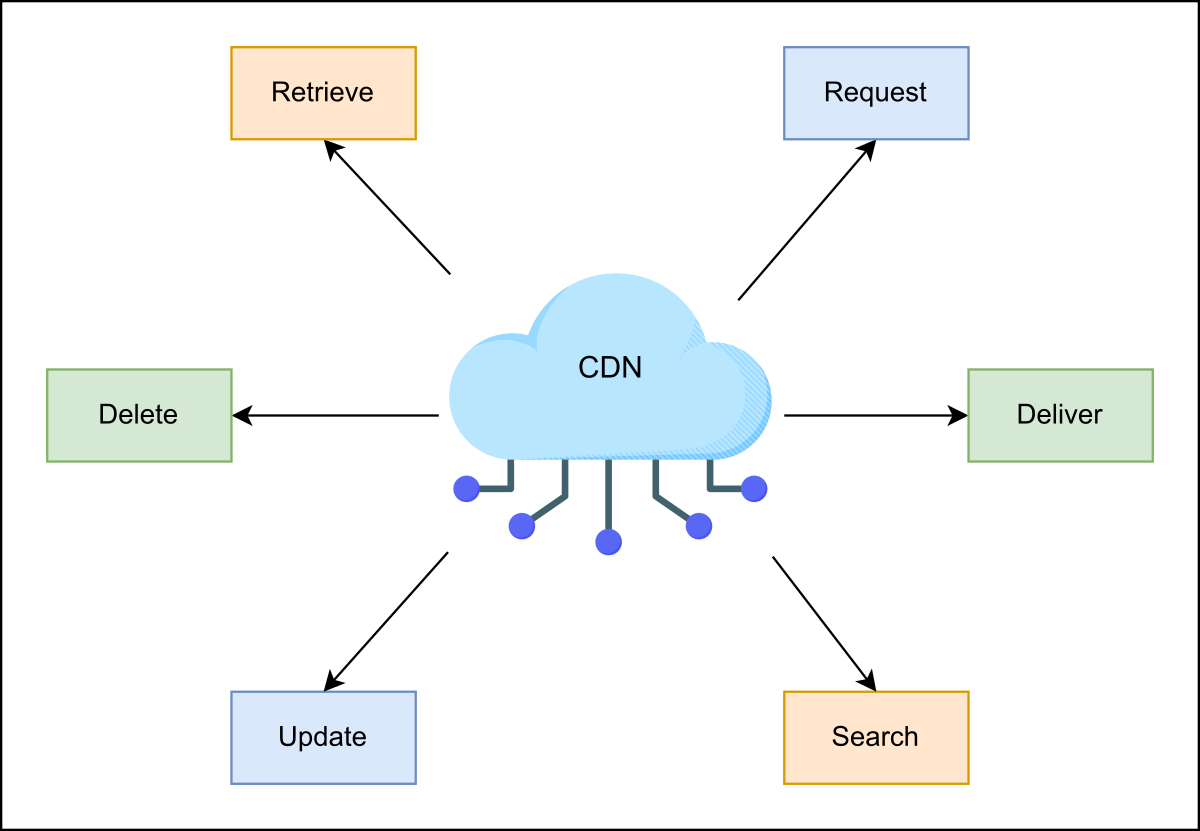
\includegraphics[width=0.5\textwidth]{Images/chapter_11/section_5560114131501056/6396621699284992.png}
 \caption{Functional requirements of a CDN}
\end{figure}

\subsubsection{Non-functional requirements}\label{wnYd-9sZij4K9w_zrJHEc}

\begin{itemize}
\item
\protect\phantomsection\label{riq23mmqMJV7QZ6h_cF5C}
\textbf{Performance}: Minimizing latency is one of the core missions of a CDN. The proposed design should have the minimum possible latency.
\item
\protect\phantomsection\label{Wl9Nq0RLt4aw6H9fD53u3}
\textbf{Availability}: CDNs are expected to be available at all times because of their effectiveness. Availability includes protection against attacks like DDoS(In DDoS attacks, malicious agents overwhelm the origin or application server by sending a massive number of requests.) and maintaining service continuity.
\item
\protect\phantomsection\label{lClhNXelkgQQhs7uyse5N}
\textbf{Scalability}: An increasing number of users will request content from CDNs. Our proposed CDN design should be able to scale horizontally as the requirements increase.
\item
\protect\phantomsection\label{FxEtpw2E1L1bVFWp0fv0p}
\textbf{Reliability and security}: Our CDN design should ensure no single point of failure. Apart from failures, the designed CDN must reliably handle massive traffic loads. Furthermore, CDNs should provide protection to hosted content from various attacks.
\end{itemize}

\begin{figure}[htbp]
 \centering
 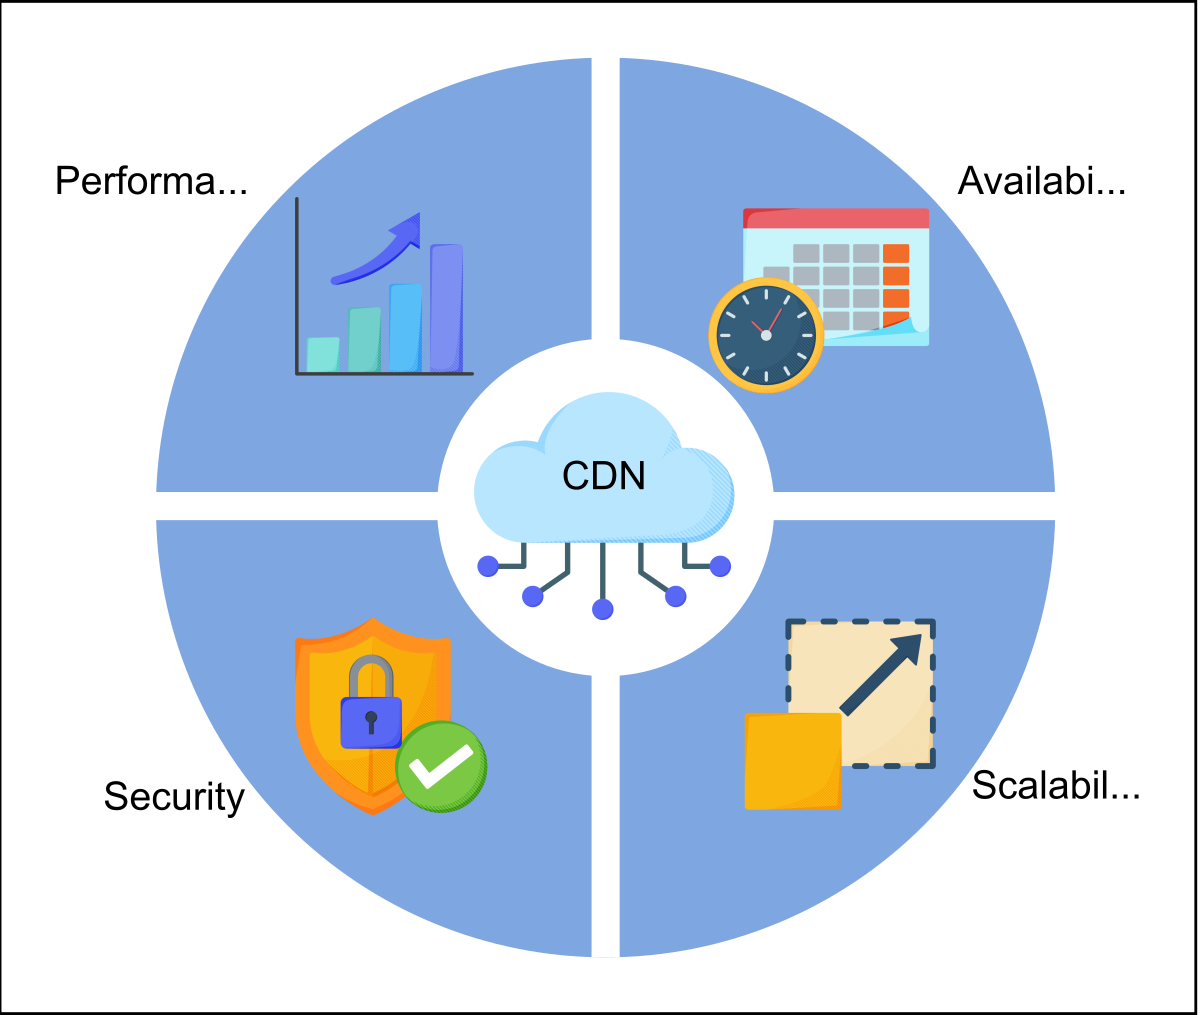
\includegraphics[width=0.5\textwidth]{Images/chapter_11/section_5560114131501056/5410676153909248.png}
 \caption{Non-functional requirements of CDN}
\end{figure}

\subsection{Building blocks we will use}\label{piacZ4l8_oyO1PNwr64YH}
\\
The design of a CDN utilizes the following building blocks:

\begin{figure}[htbp]
 \centering
 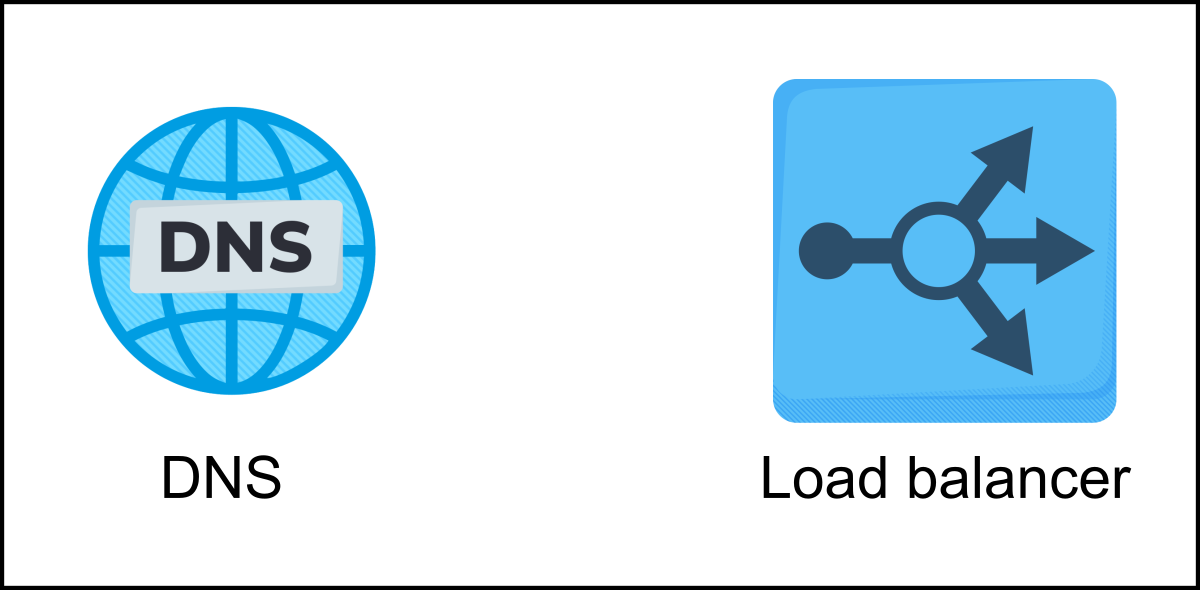
\includegraphics[width=0.5\textwidth]{Images/chapter_11/section_5560114131501056/4655970506899456.png}
 \caption{The building blocks used in CDN design}
\end{figure}

\begin{itemize}
\item
\protect\phantomsection\label{m0ufnrskIf_FA8lePpdLb}
\href{https://www.educative.io/courses/grokking-the-system-design-interview/introduction-to-domain-name-system-dns}{\textbf{DNS}} is the service that maps human-friendly CDN domain names to machine-readable IP addresses. This IP address will take the users to the specified proxy server.
\item
\protect\phantomsection\label{sIlaLphNWMr1qe68mPZ-x}
\href{https://www.educative.io/courses/grokking-the-system-design-interview/introduction-to-load-balancers}{\textbf{Load balancers}} distribute millions of requests among the operational proxy servers.
\end{itemize}
\\
In the next lesson, we'll discuss the design of the CDN.

% End of section content